% ttauto.tex -- mathematics and implementation of the pseudo-Anosov test
% in ttauto: train tracks, folds, the automaton, and the Bestvina--Handel
% gate condition as it is computed along a folding path.
%
% Build: latexmk -pdf ttauto.tex   (the PDF is not committed)
\documentclass[12pt]{amsart}
\usepackage{amsmath,amssymb,amsthm}
\usepackage[margin=1in]{geometry}
\usepackage{booktabs}
\usepackage{array}
\usepackage{tikz}
\usetikzlibrary{arrows.meta,calc,positioning,decorations.markings,shapes.misc}
\usepackage{hyperref}
\hypersetup{colorlinks=true,linkcolor=blue!60!black,citecolor=blue!60!black,
  urlcolor=blue!60!black}

% --- macros shared with the ttauto paper and the issue-2 note ---
\newcommand{\anti}[1]{\bar{#1}}          % reversed edge
\usepackage{url}
\DeclareUrlCommand\code{\urlstyle{tt}}   % breakable at / . _ :
\newcommand{\ho}{\varphi}                 % homeomorphism
\newcommand{\trk}{\tau}                   % train track
\newcommand{\Dg}{D}                       % derivative
\newcommand{\dirs}{\mathcal{E}}           % oriented edges (directions)
\newcommand{\turns}{\mathcal{T}}
\newcommand{\per}{P}                      % peripheral loop
\newcommand{\lam}{\lambda}
\newcommand{\np}{n}                       % number of punctures
\newcommand{\ttauto}{\texttt{ttauto}}
\newcommand{\set}[1]{\{#1\}}

\theoremstyle{plain}
\newtheorem{Theorem}{Theorem}[section]
\newtheorem{Proposition}[Theorem]{Proposition}
\newtheorem{Lemma}[Theorem]{Lemma}
\newtheorem{Corollary}[Theorem]{Corollary}
\theoremstyle{definition}
\newtheorem{Definition}[Theorem]{Definition}
\newtheorem{Remark}[Theorem]{Remark}
\newtheorem{Example}[Theorem]{Example}

\tikzset{
  main/.style={thick},
  side/.style={thick,blue!70!black},
  periph/.style={thick,red!70!black},
  image/.style={very thick,orange!90!black,-{Stealth[length=2.5mm]}},
  gate/.style={line width=2.5pt,gray!60,line cap=round},
  chord/.style={thick,dashed},
  vert/.style={circle,fill=black,inner sep=1.2pt},
  punct/.style={circle,fill=black,inner sep=1.6pt},
  pr/.style={font=\scriptsize,gray!60!black},   % prong numbers
  lbl/.style={font=\small},
  state/.style={circle,draw,thick,minimum size=8mm,inner sep=0pt},
  branch/.style={thick,-{Stealth[length=2.5mm]}},
  cyc/.style={very thick,orange!90!black,-{Stealth[length=2.5mm]}},
  oriented/.style={main,postaction={decorate},
    decoration={markings,mark=at position 0.55 with {\arrow{Stealth[length=2mm]}}}},
  disc/.style={thick,gray!70},
}

\title[The pseudo-Anosov test in \ttauto]{\ttauto: mathematics and
  implementation of the pseudo-Anosov test}
\date{19 September 2026.  Describes the code at commit \code{bb29dc5}.}

\begin{document}

\begin{abstract}
  \ttauto\ enumerates pseudo-Anosov homeomorphisms of the punctured disc
  as closed paths in a folding automaton of train tracks.  This document
  explains, for a reader who knows train tracks but not the code, what
  the library computes and why it is correct: how a track is encoded and
  numbered, what one fold does to the edges as a matrix and as a
  free-group substitution, how the automaton and the search are built on
  that, and above all how the Bestvina--Handel criterion for
  pseudo-Anosov (a primitive transition matrix \emph{and} connected gates
  at every vertex) is evaluated along a folding path without ever writing
  down an image word.  A four-puncture example is worked out completely,
  from the four one-step maps to the gate graph that shows the map to be
  reducible.  An appendix maps each concept to the file that implements
  it and the test that pins it.
\end{abstract}

\maketitle
\tableofcontents

\subsection*{A note about numbering}
There is an inherent tension present in the code: mathematical objects are
usually numbered from~$1$ in the literature, but the C++ language is
zero-indexed (the first element of an array is zero).  These two conventions
coexist here, and the loose rule is that user-facing objects are numbered
from~$1$, while the internals are numbered from~$0$.
\begin{itemize}
  \item \textbf{One-indexed}: everything a user reads or types.  The
    interactive \code{ttauto} program numbers strata, subautomata and
    vertices from~$1$, as do its Mathematica output files and the printed
    codings.  The \emph{letters} are also one-indexed, of necessity.  A
    train-track map is stored as a substitution on an alphabet whose
    letters are signed integers naming the edges and sides of the track
    (Section~\ref{sec:onefold}); the sign carries the orientation
    ($\anti e=-e$), so zero cannot be a letter.
  \item \textbf{Zero-indexed}: everything inside the library.  Vertices
    and branches of the automaton, multigons, prongs, edges and fold
    indices are C++ indices from~$0$, and so are the diagnostic printouts
    of the library itself (the gate table, the fold record, the path lists
    of the search).
\end{itemize}

%======================================================================
\section{Train tracks and their numbering}
\label{sec:tracks}

\subsection{Multigons, prongs, cusps}
The surface throughout is the disc with $\np$ punctures, $\np\ge3$, and
the train tracks are the properly embedded ones of \cite{Lanneau2011}.
A train track in \ttauto\ is a finite list of \emph{multigons}.  A
multigon with $k$ prongs is a $k$-gon whose $k$ corners are the
\emph{prongs}; at each prong a linearly ordered list of \emph{main edges}
is attached, and two consecutive edges at the same prong form a
\emph{cusp}.  The $k$ \emph{sides} of the polygon are infinitesimal: they
carry no weight and are never folded.  A multigon may be \emph{punctured};
a punctured monogon ($k=1$) is the standard neighbourhood of a puncture,
its single side is a loop around the puncture.  Properly embedded means
that every puncture is enclosed by a punctured monogon and that the track
fills the disc: its complement consists of the interiors of the polygons
and of the punctured monogons, and one more region, the annulus between
the track and the outer boundary of the disc.  Every edge has two ends
attached at prongs, so the structure is a graph whose vertices are
blown up into polygons (Figure~\ref{fig:multigon}).  The corners of the
boundary region are the cusps of the track, so that region is a polygon
with as many prongs as the track has cusps.  The \emph{singularity data}
of a track lists its multigons with their prong numbers, a dot marking
the punctured ones, and the number of cusps in parentheses;
Figure~\ref{fig:tracks} shows the tracks $1.\,1.\,1.\,1.\,(2)$, four
punctured monogons and a 2-pronged boundary, and $1.\,1.\,1.\,1.\,3\,(1)$,
which has in addition an unpunctured trigon and a 1-pronged boundary.
Tracks with the same singularity data form a \emph{stratum}, and the
constructor \code{build_traintrack_list(n)} returns one representative
track per stratum of the disc with $n$ punctures.

\begin{figure}[t]
  \centering
  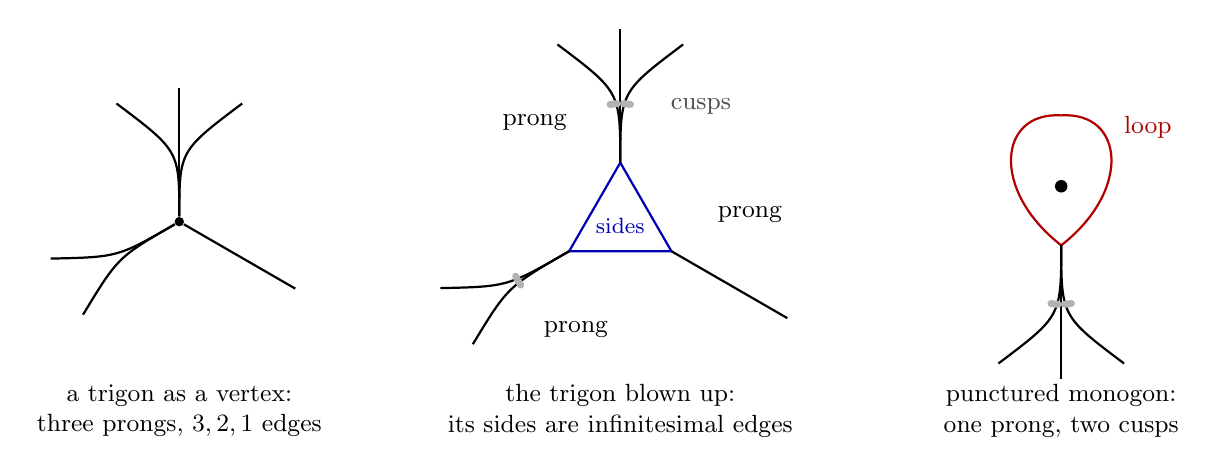
\begin{tikzpicture}[scale=1.0]
    % ---- left: the multigon as a vertex of the graph ----
    \begin{scope}
      \node[vert] (v) at (0,0) {};
      \foreach \a in {62,90,118} \draw[main] (v) .. controls (90:0.9) .. (\a:1.7);
      \foreach \a in {196,224} \draw[main] (v) .. controls (210:0.9) .. (\a:1.7);
      \draw[main] (v) -- (330:1.7);
      \node[lbl,align=center] at (0,-2.4) {a trigon as a vertex:\\ three prongs, $3,2,1$ edges};
    \end{scope}
    % ---- middle: the same multigon blown up into a trigon ----
    \begin{scope}[xshift=5.6cm]
      \coordinate (A) at (90:0.75);
      \coordinate (B) at (210:0.75);
      \coordinate (C) at (330:0.75);
      \draw[side] (A) -- (B) -- (C) -- cycle;
      \foreach \a in {62,90,118} \draw[main] (A) .. controls ($(A)+(90:0.9)$) .. ($(A)+(\a:1.7)$);
      \foreach \a in {196,224} \draw[main] (B) .. controls ($(B)+(210:0.9)$) .. ($(B)+(\a:1.7)$);
      \draw[main] (C) -- ($(C)+(330:1.7)$);
      % cusps: the thin wedges between consecutive tangent edges
      \draw[gate] ($(A)+(80:0.75)$) arc (80:87:0.75);
      \draw[gate] ($(A)+(93:0.75)$) arc (93:100:0.75);
      \draw[gate] ($(B)+(205:0.75)$) arc (205:215:0.75);
      \node[lbl,gray!60!black] at ($(A)+(35:1.25)$) {cusps};
      \node[lbl] at ($(A)+(155:1.2)$) {prong};
      \node[lbl] at ($(C)+(25:1.1)$) {prong};
      \node[lbl] at ($(B)+(275:1.0)$) {prong};
      \node[lbl,blue!70!black,align=center] at (0,-0.05) {\footnotesize sides};
      \node[lbl,align=center] at (0,-2.4) {the trigon blown up:\\ its sides are infinitesimal edges};
    \end{scope}
    % ---- right: a punctured monogon ----
    \begin{scope}[xshift=11.2cm]
      \coordinate (c) at (0,-0.3);
      \node[punct] at (0,0.45) {};
      \draw[periph] (c) .. controls (-0.9,0.4) and (-0.8,1.4) .. (0,1.35)
                        .. controls (0.8,1.4) and (0.9,0.4) .. (c);
      \foreach \a in {242,270,298} \draw[main] (c) .. controls ($(c)+(270:0.9)$) .. ($(c)+(\a:1.7)$);
      \draw[gate] ($(c)+(260:0.75)$) arc (260:267:0.75);
      \draw[gate] ($(c)+(273:0.75)$) arc (273:280:0.75);
      \node[lbl,red!70!black] at (1.1,1.2) {loop};
      \node[lbl,align=center] at (0,-2.4) {punctured monogon:\\ one prong, two cusps};
    \end{scope}
  \end{tikzpicture}
  \caption{Left: a trigon drawn as a vertex of the underlying graph.  It
    has three prongs, each a bundle of edges that are mutually tangent
    where they meet the vertex, with $3$, $2$ and $1$ edges.  Middle: the
    same trigon blown up, as \ttauto\ stores it: the blue sides are
    infinitesimal edges, and consecutive edges at one prong are separated
    by a cusp, the thin wedge between two tangent edges.  Right: a
    punctured monogon, whose single side is the loop around the puncture
    (the dot).}
  \label{fig:multigon}
\end{figure}

\begin{figure}[t]
  \centering
  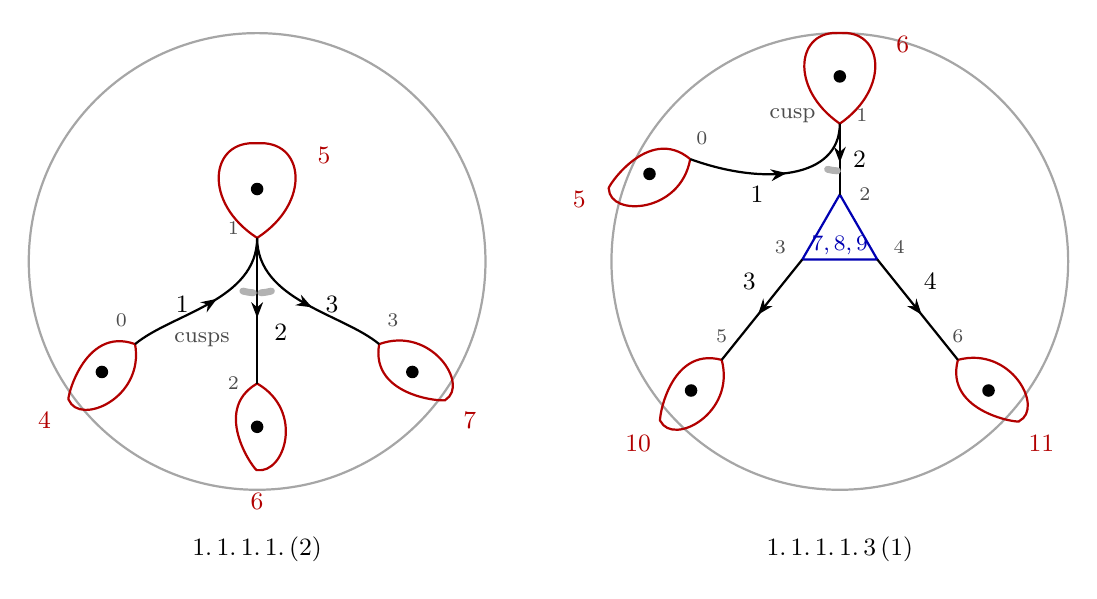
\begin{tikzpicture}[scale=1.0]
    % ---------- left: 1.1.1.1.(2), the vertex-0 track of Section 5 ----------
    \begin{scope}
      \draw[disc] (0,-0.3) circle (2.9);
      % monogon 3 (prong 1) at the centre, loop 5 above, puncture inside
      \coordinate (p1) at (0,0);
      \node[punct] at (0,0.62) {};
      \draw[periph] (p1) .. controls (0.7,0.45) and (0.6,1.25) .. (0,1.2)
                       .. controls (-0.6,1.25) and (-0.7,0.45) .. (p1);
      \node[lbl,red!70!black] at (0.85,1.05) {$5$};
      % monogon 0 (prong 0), lower left, loop 4 beyond the prong point
      \coordinate (p0) at (-1.55,-1.35);
      \node[punct] at ($(p0)+(220:0.55)$) {};
      \draw[periph] (p0) .. controls ($(p0)+(160:0.7)$) and ($(p0)+(220:1.15)$) .. ($(p0)+(220:1.1)$)
                       .. controls ($(p0)+(220:1.15)+(300:0.35)$) and ($(p0)+(280:0.7)$) .. (p0);
      \node[lbl,red!70!black] at ($(p0)+(220:1.5)$) {$4$};
      % monogon 1 (prong 2), bottom, loop 6
      \coordinate (p2) at (0,-1.85);
      \node[punct] at ($(p2)+(270:0.55)$) {};
      \draw[periph] (p2) .. controls ($(p2)+(210:0.7)$) and ($(p2)+(270:1.15)$) .. ($(p2)+(270:1.1)$)
                       .. controls ($(p2)+(270:1.15)+(0:0.35)$) and ($(p2)+(330:0.7)$) .. (p2);
      \node[lbl,red!70!black] at ($(p2)+(270:1.5)$) {$6$};
      % monogon 2 (prong 3), lower right, loop 7
      \coordinate (p3) at (1.55,-1.35);
      \node[punct] at ($(p3)+(320:0.55)$) {};
      \draw[periph] (p3) .. controls ($(p3)+(260:0.7)$) and ($(p3)+(320:1.15)$) .. ($(p3)+(320:1.1)$)
                       .. controls ($(p3)+(320:1.15)+(40:0.35)$) and ($(p3)+(20:0.7)$) .. (p3);
      \node[lbl,red!70!black] at ($(p3)+(320:1.5)$) {$7$};
      % edges: 1 from prong 0 to prong 1, 2 from prong 1 to prong 2, 3 from prong 1 to prong 3
      \draw[oriented] (p0) .. controls ($(p0)+(40:0.6)$) and ($(p1)+(270:0.8)$) .. (p1);
      \draw[oriented] (p1) -- (p2);
      \draw[oriented] (p1) .. controls ($(p1)+(270:0.8)$) and ($(p3)+(140:0.6)$) .. (p3);
      \node[lbl] at (-0.95,-0.85) {$1$};
      \node[lbl] at (0.3,-1.2) {$2$};
      \node[lbl] at (0.95,-0.85) {$3$};
      % prong numbers
      \node[pr] at (-0.3,0.12) {1};
      \node[pr] at ($(p0)+(120:0.35)$) {0};
      \node[pr] at ($(p2)+(180:0.3)$) {2};
      \node[pr] at ($(p3)+(60:0.35)$) {3};
      % cusps at prong 1: thin wedges between the tangent edges
      \draw[gate] (255:0.7) arc (255:266:0.7);
      \draw[gate] (274:0.7) arc (274:285:0.7);
      \node[lbl,gray!60!black] at (-0.7,-1.3) {\footnotesize cusps};
      \node[lbl] at (0,-3.95) {$1.\,1.\,1.\,1.\,(2)$};
    \end{scope}
    % ---------- right: 1.1.1.1.3(1) ----------
    \begin{scope}[xshift=7.4cm]
      \draw[disc] (0,-0.3) circle (2.9);
      % trigon (multigon 4) at the centre: prongs 2 (top), 3 (lower left), 4 (lower right)
      \coordinate (q2) at (90:0.55);
      \coordinate (q3) at (210:0.55);
      \coordinate (q4) at (330:0.55);
      \draw[side] (q2) -- (q3) -- (q4) -- cycle;
      \node[lbl,blue!70!black] at (0,-0.1) {\footnotesize $7,8,9$};
      % monogon 3 (prong 1) above the trigon, loop 6 above it; two edges: 1 in, 2 out
      \coordinate (p1) at (0,1.45);
      \node[punct] at (0,2.05) {};
      \draw[periph] (p1) .. controls (0.65,1.9) and (0.55,2.65) .. (0,2.6)
                       .. controls (-0.55,2.65) and (-0.65,1.9) .. (p1);
      \node[lbl,red!70!black] at (0.8,2.45) {$6$};
      % monogon 0 (prong 0) to the left, loop 5
      \coordinate (p0) at (-1.9,1.0);
      \node[punct] at ($(p0)+(200:0.55)$) {};
      \draw[periph] (p0) .. controls ($(p0)+(140:0.7)$) and ($(p0)+(200:1.15)$) .. ($(p0)+(200:1.1)$)
                       .. controls ($(p0)+(200:1.15)+(280:0.35)$) and ($(p0)+(260:0.7)$) .. (p0);
      \node[lbl,red!70!black] at ($(p0)+(200:1.5)$) {$5$};
      % monogon 1 (prong 5) lower left, loop 10; monogon 2 (prong 6) lower right, loop 11
      \coordinate (p5) at (-1.5,-1.55);
      \node[punct] at ($(p5)+(225:0.55)$) {};
      \draw[periph] (p5) .. controls ($(p5)+(165:0.7)$) and ($(p5)+(225:1.15)$) .. ($(p5)+(225:1.1)$)
                       .. controls ($(p5)+(225:1.15)+(305:0.35)$) and ($(p5)+(285:0.7)$) .. (p5);
      \node[lbl,red!70!black] at ($(p5)+(225:1.5)$) {$10$};
      \coordinate (p6) at (1.5,-1.55);
      \node[punct] at ($(p6)+(315:0.55)$) {};
      \draw[periph] (p6) .. controls ($(p6)+(255:0.7)$) and ($(p6)+(315:1.15)$) .. ($(p6)+(315:1.1)$)
                       .. controls ($(p6)+(315:1.15)+(35:0.35)$) and ($(p6)+(15:0.7)$) .. (p6);
      \node[lbl,red!70!black] at ($(p6)+(315:1.5)$) {$11$};
      % edges: 1: prong 0 -> prong 1; 2: prong 1 -> prong 2; 3: prong 3 -> prong 5; 4: prong 4 -> prong 6
      \draw[oriented] (p0) .. controls ($(p0)+(340:1.0)$) and ($(p1)+(270:0.7)$) .. (p1);
      \draw[oriented] (p1) -- (q2);
      \draw[oriented] (q3) -- (p5);
      \draw[oriented] (q4) -- (p6);
      \node[lbl] at (-1.05,0.55) {$1$};
      \node[lbl] at (0.25,1.0) {$2$};
      \node[lbl] at (-1.15,-0.55) {$3$};
      \node[lbl] at (1.15,-0.55) {$4$};
      % prong numbers
      \node[pr] at ($(p0)+(60:0.3)$) {0};
      \node[pr] at ($(p1)+(20:0.3)$) {1};
      \node[pr] at ($(q2)+(0:0.32)$) {2};
      \node[pr] at ($(q3)+(150:0.32)$) {3};
      \node[pr] at ($(q4)+(30:0.32)$) {4};
      \node[pr] at ($(p5)+(90:0.3)$) {5};
      \node[pr] at ($(p6)+(90:0.3)$) {6};
      % cusp at prong 1 between edges 1 and 2
      \draw[gate] ($(p1)+(255:0.6)$) arc (255:267:0.6);
      \node[lbl,gray!60!black] at (-0.6,1.55) {\footnotesize cusp};
      \node[lbl] at (0,-3.95) {$1.\,1.\,1.\,1.\,3\,(1)$};
    \end{scope}
  \end{tikzpicture}
  \caption{Two properly embedded train tracks on the disc with four
    punctures, with their canonical numbering.  Punctures are dots,
    loops of punctured monogons are red and labelled by their side
    letter, main edges are black with their orientation and number, sides
    of the unpunctured trigon are blue, and the small grey numbers are the
    prong numbers.  Left: the stratum $1.\,1.\,1.\,1.\,(2)$
    (vertex~0 of Section~\ref{sec:example}); the central monogon carries
    three edges and two cusps, so the region between the track and the
    grey boundary has two prongs.  Right: the stratum $1.\,1.\,1.\,1.\,3\,(1)$,
    with an unpunctured trigon and a single cusp.}
  \label{fig:tracks}
\end{figure}


\subsection{Codings and normal form}
A track is identified up to isotopy by its \emph{coding}: a depth-first
walk that starts at an uncusped monogon (a punctured monogon carrying a
single edge), crosses its edge, and at every multigon it enters records
the number of prongs, the puncture label, the entry prong and the number
of edges at each prong, descending into each edge in the cyclic order of
the prongs and of the slots at a prong.  The walk from a fixed start is
deterministic, so the coding is a function of the start monogon;
\code{normalise()} rotates every multigon to a canonical position,
sorts the multigons, and moves to slot~$0$ the uncusped monogon whose
coding is lexicographically smallest.  After normalisation
\code{coding()} is that minimal coding, two tracks are equal
(\code{operator==}) if and only if their codings are equal, and
\code{traintrack(code)} rebuilds a track from its coding.  The mirror
image has coding \code{coding(-1)}, the same walk run in the opposite
cyclic direction; a track is \emph{reflection symmetric} when the two
agree.  A track is \emph{cyclically symmetric} when several uncusped
monogons give the same minimal coding; \code{cyclic_symmetry()} returns
the induced permutation of the edges.

\subsection{The canonical numbering}
\label{sec:numbering}
Everything the maps below say about a track is expressed in one
\emph{numbering} of its prongs, edges and cusps, the struct
\code{ttnumbering} returned by \code{traintrack::numbering()}.  It is
produced by the same walk as the coding, started at monogon~$0$:
\begin{itemize}
  \item prongs are numbered $0,1,2,\dots$ in the order the walk first
    reaches them; when the walk enters a $k$-gon at prong $p$ it numbers
    all $k$ prongs consecutively from $p$ in the cyclic direction;
  \item edges are numbered in the order the walk first crosses them, and
    each edge is oriented \emph{away} from the multigon that first
    reaches it, so an edge has a tail prong and a head prong
    (\code{edge_tail}, \code{edge_head});
  \item side $q$ is the side that runs from prong $q$ to the next prong
    of the same multigon in the cyclic direction (for a monogon, its loop);
  \item cusps are listed in the order the walk meets them, and fold index
    $f$ refers to cusp $\lfloor f/2\rfloor$ folded in direction
    $1-2(f\bmod 2)$.
\end{itemize}
This is exactly the order in which \code{weights()} reads the edge
weights, so the rows and columns of every transition matrix are indexed
by edge numbers.  The numbering also carries the list of prong letters
(\code{prong_letters[q]}: the signed main letters whose tail is at prong
$q$), the type of each prong (\code{nprongs}, \code{punctured}) and the
letter conventions \code{main_letter(e)}${}=e+1$ and
\code{side_letter(q)}${}=n+1+q$.

Because the walk is determined by the coding, the numbering is a function
of the coding: two normalised tracks with the same coding have the same
edge tails and heads, prong letters and cusps (\code{same_labels}).
Section~\ref{sec:labels} explains why this is what makes the automaton
compose maps across vertices without any transport step.

%======================================================================
\section{Folds, the automaton, and the search}
\label{sec:folds}

\subsection{One fold}
\label{sec:onefold}
A fold takes a cusp, that is two consecutive edges $e_0$ and $e_1$ at the
same prong of a multigon $M$, and folds $e_0$ onto $e_1$
(Figure~\ref{fig:fold}).  Let the other end of $e_1$ be at prong $t$ of
the \emph{target} multigon $T$, which has $k$ prongs.  The fold is legal
when $e_1$ is the outermost edge at $t$ on the appropriate side; the end
of $e_0$ at $M$ is then detached, slid along $e_1$ to $T$, carried along
the side of $T$ from $t$ to the adjacent prong $t'=t\pm1 \pmod k$, and
re-attached there as the outermost edge.  For a punctured monogon target,
$k=1$, $t'=t$ and the edge goes once around the puncture.  Finally the
track is normalised.  Folds never create or destroy prongs or edges, so
the singularity data is preserved and the prongs before and after a fold
are in canonical bijection.

\begin{figure}[t]
  \centering
  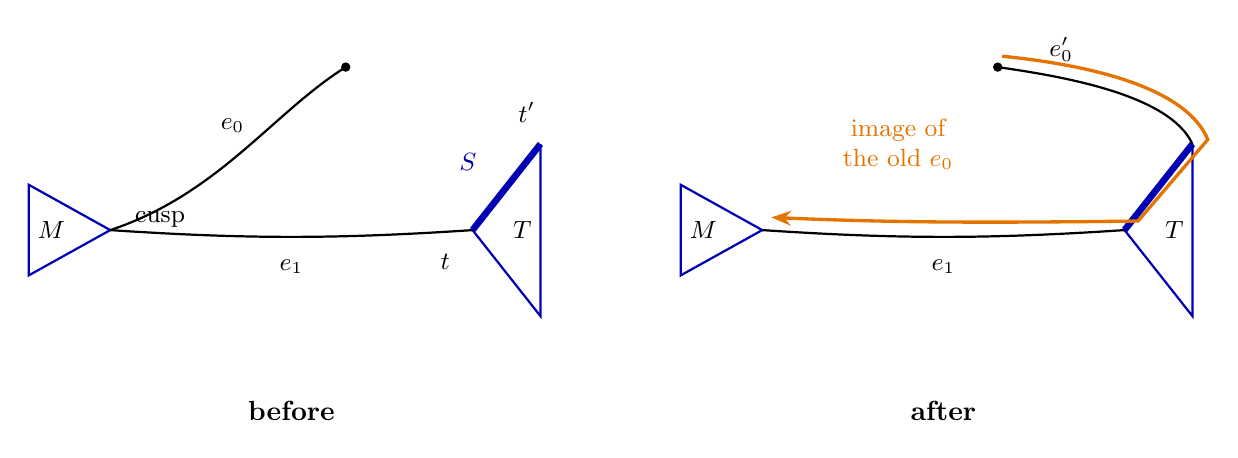
\begin{tikzpicture}[scale=1.15]
    \begin{scope}
      \coordinate (m0) at (0,0);
      \coordinate (m1) at (-0.9,0.5);
      \coordinate (m2) at (-0.9,-0.5);
      \draw[side] (m0) -- (m1) -- (m2) -- cycle;
      \node[lbl] at (-0.65,0) {$M$};
      \coordinate (t0) at (4,0);
      \coordinate (t1) at (4.75,0.95);
      \coordinate (t2) at (4.75,-0.95);
      \draw[side] (t0) -- (t2) -- (t1);
      \draw[side,line width=2.4pt] (t0) -- (t1);
      \node[lbl] at (4.55,0) {$T$};
      \node[lbl] at (3.7,-0.35) {$t$};
      \node[lbl] at (4.6,1.3) {$t'$};
      \node[lbl,blue!70!black] at (3.95,0.75) {$S$};
      \draw[main] (m0) .. controls (1.5,-0.1) and (2.5,-0.1) .. (t0);
      \node[lbl] at (2,-0.4) {$e_1$};
      \draw[main] (m0) .. controls (1.2,0.4) and (1.8,1.3) .. (2.6,1.8);
      \node[vert] at (2.6,1.8) {};
      \node[lbl] at (1.35,1.15) {$e_0$};
      \node[lbl] at (0.55,0.12) {cusp};
      \node at (2,-2.0) {\textbf{before}};
    \end{scope}
    \begin{scope}[xshift=7.2cm]
      \coordinate (m0) at (0,0);
      \coordinate (m1) at (-0.9,0.5);
      \coordinate (m2) at (-0.9,-0.5);
      \draw[side] (m0) -- (m1) -- (m2) -- cycle;
      \node[lbl] at (-0.65,0) {$M$};
      \coordinate (t0) at (4,0);
      \coordinate (t1) at (4.75,0.95);
      \coordinate (t2) at (4.75,-0.95);
      \draw[side] (t0) -- (t2) -- (t1);
      \draw[side,line width=2.4pt] (t0) -- (t1);
      \node[lbl] at (4.55,0) {$T$};
      \draw[main] (m0) .. controls (1.5,-0.1) and (2.5,-0.1) .. (t0);
      \node[lbl] at (2,-0.4) {$e_1$};
      \draw[main] (2.6,1.8) .. controls (3.3,1.7) and (4.5,1.5) .. (t1);
      \node[vert] at (2.6,1.8) {};
      \node[lbl] at (3.3,2.0) {$e_0'$};
      \draw[image] (2.65,1.92) .. controls (3.35,1.85) and (4.65,1.65) .. (4.92,1.0)
        -- (4.15,0.1) .. controls (2.5,0.08) and (1.5,0.08) .. (0.1,0.14);
      \node[lbl,orange!90!black,align=center] at (1.5,0.95) {image of\\ the old $e_0$};
      \node at (2,-2.0) {\textbf{after}};
    \end{scope}
  \end{tikzpicture}
  \caption{Folding $e_0$ onto $e_1$ at a cusp of the multigon $M$.  The
    end of $e_0$ at $M$ slides along $e_1$ to the target multigon $T$,
    arriving at prong $t$, and then along the side $S$ of $T$ to the
    adjacent prong $t'$, where it re-attaches.  The image of the old edge
    $e_0$, oriented from its far end towards $M$, is the path
    $e_0'\,S\,e_1$.  The side traversed belongs to the \emph{target}
    multigon.}
  \label{fig:fold}
\end{figure}

The library records what one fold does in a \code{fold_map_data}
(filled by \code{traintrack::fold_with_map}), entirely in the
numberings before and after the fold: the old edge numbers
\code{moved}${}=e_0$ and \code{onto}${}=e_1$; the direction; the cusp
prong; the target prongs $t$ (\code{target_from}) and $t'$
(\code{target_to}); the signed side letter $S$ traversed between them;
\code{edge_image[e]}, the signed new letter of every old edge $e$ (the
sign records whether the canonical orientations before and after agree);
\code{prong_image[q]}, the new number of old prong $q$; and the
three-letter word \code{moved_word} which is the image of $e_0$.  Two
algebraic objects are read off the record.

\paragraph{The train-track map.}
The one-fold map is a substitution on the $n+n_{\mathrm{s}}$ letters
(\code{fold_map_data::to_freeauto}, a \code{jlt::freeauto<int>}): every
edge other than $e_0$ goes to its signed new letter, every side goes to
its new side, and $e_0$, in its canonical orientation, goes to
\[
  e_0 \;\longmapsto\; e_0'\;S\;e_1
  \qquad\text{or}\qquad
  e_0 \;\longmapsto\; \anti{e_1}\;\anti S\;\anti{e_0'},
\]
depending on which end of $e_0$ was at the cusp.  Inverses act on words
in the usual way, so every image word is an edge path in the new track:
consecutive letters share a prong, and the side letter between two main
letters is the side of the target multigon that the path runs along.

\paragraph{The transition matrix.}
Its abelianisation on main edges is the $n\times n$ matrix with
$M_{e'e}=$ number of times $e'$ occurs in the image of $e$, regardless of
sign; for one fold this is a permutation matrix plus a single extra $1$
in the row of $e_1'$ and the column of $e_0$
(\code{fold_map_data::transition_matrix}, stored as a
\code{mathmatrix_permplus1}).  Composing folds multiplies matrices:
$M(\gamma)=M_L\cdots M_2M_1$ for a path of $L$ folds, so
$M(\gamma)_{e'e}$ counts how many times the image of $e$ crosses $e'$.

\subsection{The automaton}
The \emph{folding automaton} of a stratum (\code{ttfoldgraph}) has one
vertex per normalised track and one branch per legal fold.  It is built
recursively from a starting track: every fold index is tried, the result
is normalised, identified with an existing vertex if its coding is
already present and added otherwise, and the branch stores the target
vertex, the one-step transition matrix and the one-step map
(\code{target_vertex}, \code{transition_matrix}, \code{traintrack_map}).
Folds that are not legal are skipped, and a fold whose matrix is the
identity contributes no branch.  The automaton usually decomposes into
strongly connected components (\code{subgraphs}); the searches below run
on the \emph{main} component, the one that contains pseudo-Anosovs.  A
\code{folding_path} is a start vertex and a sequence of branch choices;
it composes the stored one-step data into the path matrix
(\code{transition_matrix()}), the path map (\code{traintrack_map()}),
the sequence of vertices visited, and knows whether it is closed.  Two
closed paths are equal when they are cyclic rotations of each other.

\subsection{The search}
\label{sec:search}
\code{ttauto::ttauto::search()} performs a depth-first search over
folding paths from every vertex of the automaton (skipping one vertex of
each reflection-symmetric pair, since the mirror image gives the same
dilatations).  Partial paths are pruned by a length bound
(\code{max_pathlength}) or, in the norm-bounded mode
(\code{check_norms}), as soon as the minimum row or column sum of the
running matrix exceeds the dilatation being searched for, since that sum
is a lower bound on the spectral radius and grows along the path.
Optionally \emph{bad words} (\code{badwords}) are pruned: closed subpaths
whose matrix has the same zero pattern as its square can be traversed
once instead of repeatedly without lowering the dilatation.  When a path
closes, \code{record_pA} decides whether it is a pseudo-Anosov
(Section~\ref{sec:criterion}); accepted paths are grouped into
\code{pAclass} objects keyed by characteristic polynomial, and each class
keeps its dilatation and a few representative paths.  Rejected
candidates go to a second list.

%======================================================================
\section{When is a closed path pseudo-Anosov?}
\label{sec:criterion}

A closed folding path $\gamma$ of length $L$ from a track $\trk$ back to
$\trk$ defines a homeomorphism $\ho$ of the punctured disc, up to
isotopy: perform the $L$ folds and identify the final track with $\trk$
by the canonical numbering.  The train-track map $g=g(\gamma)$ carries
$\trk$ to itself; its main-edge matrix is $M(\gamma)$.  The question is
when $\ho$ is pseudo-Anosov, and then its dilatation is the
Perron--Frobenius eigenvalue of $M(\gamma)$.

\subsection{Matrix conditions, and why they are not enough}
Two conditions on $M(\gamma)$ are necessary.  It must be
\emph{irreducible}: an invariant proper subset of edges would carry an
invariant subgraph, hence a reduction.  Its spectral radius $\lam$ must
exceed $1$: otherwise the growth is polynomial and $\ho$ is reducible or
finite order.  \ttauto\ in fact requires the stronger property that
$M(\gamma)$ be \emph{primitive}, some power strictly positive
(\code{is_primitive}), for the following reason.

\begin{Remark}[primitive versus irreducible]
  \label{rem:primitive}
  An irreducible non-negative matrix of period $p>1$ has $p$ eigenvalues
  of modulus $\lam$, namely $\lam$ times the $p$th roots of unity, and no
  strictly positive power.  Such a matrix does occur in the automaton:
  on the six-puncture stratum $4\,(2)$ there are closed paths whose
  characteristic polynomial is a polynomial in $x^2$, with eigenvalues
  $\pm\lam$.  The transition matrix of a pseudo-Anosov train-track map
  is primitive (its Perron root is simple and dominates), so these are
  never pseudo-Anosov, and a search that only tests irreducibility lists
  them with a spurious ``dilatation''.  Primitivity is tested by
  squaring: a non-negative $n\times n$ irreducible matrix is primitive
  iff $M^{n^2-2n+2}>0$.
\end{Remark}

Primitivity and $\lam>1$ are still not sufficient.  The matrix only sees
how many times image paths cross each edge; it does not see how those
paths turn at the vertices, and a reducing curve can hide in a vertex.
The missing condition is Bestvina and Handel's.

\subsection{Derivative, gates, infinitesimal edges}
Let $G$ be the graph underlying $\trk$ (multigons collapsed to points) and
$g\colon G\to G$ the graph map, sending edges to edge paths.  Write
$\dirs$ for the set of \emph{directions}, oriented edges of $G$; each edge
$e$ gives two directions $e$ and $\anti e$, and the directions with
initial vertex $v$ form the link of $v$ with its cyclic order.

\begin{Definition}[derivative, gates; {\cite[\S1]{Bestvina1995}}]
  The \emph{derivative} $\Dg g\colon\dirs\to\dirs$ sends a direction $E$
  to the first edge of the edge path $g(E)$.  Two directions at the same
  vertex are \emph{equivalent} if some power of $\Dg g$ identifies them;
  the classes are the \emph{gates}.  Each gate is a consecutive block in
  the cyclic order at its vertex, and distinct gates map to distinct
  gates.
\end{Definition}

An edge path $E_1E_2\cdots E_m$ passes through a vertex between $E_i$ and
$E_{i+1}$ by the pair of directions $(\anti{E_i},E_{i+1})$, a \emph{turn}.
The map is \emph{efficient} \cite[Lemma~3.1.2]{Bestvina1995} when no
image $g(E)$ backtracks and every turn it takes joins distinct gates;
then no iterate $g^k(E)$ backtracks either.

\begin{Definition}[the Bestvina--Handel train track; {\cite[\S3.3]{Bestvina1995}}]
  Around each vertex $v$ draw a small circle with one point per gate.
  The real edges of $G$ attach at the points of their gates.  Join two
  gate points by an \emph{infinitesimal edge} if and only if for some edge
  $e$ and some $m>0$ the path $g^m(e)$ takes the turn joining those two
  gates.  The result is the train track $\trk_g$, and $g$ induces a map on
  it: real edges go to their image paths with the infinitesimal edges
  inserted at the turns, infinitesimal edges to infinitesimal edges.
\end{Definition}

\begin{Theorem}[{\cite[Prop.~3.3.2, Thm.~3.1.4, Thm.~4.1.4]{Bestvina1995}}]
  \label{thm:bh}
  Let $g$ be efficient with irreducible transition matrix and $\lam>1$.
  If at some vertex the infinitesimal edges fail to connect all the
  gates, then $\ho$ is isotopic to a reducible homeomorphism: the regular
  neighbourhood of $\trk_g$ has an essential non-peripheral boundary
  component.  If at every vertex the infinitesimal edges connect all the
  gates, then $\trk_g$ is a Thurston train track, and $\ho$ is
  pseudo-Anosov with dilatation $\lam$ (on the punctured surface, with
  the peripheral edges of Section~\ref{sec:punctures} given length zero).
\end{Theorem}

So for an efficient irreducible map the matrix decides nothing further
and the gate graphs decide everything.  The paper also constrains what
the infinitesimal edges can look like in the pseudo-Anosov case, which
the implementation uses as a sanity check:

\begin{Proposition}[{\cite[Props.~3.3.3--3.3.4]{Bestvina1995}}]
  \label{prop:shape}
  If $\ho$ is pseudo-Anosov as above, every vertex has at least two
  gates, and at a vertex with $k$ gates the infinitesimal edges form the
  single edge ($k=2$), a $k$-gon joining cyclically adjacent gates, or a
  $k$-gon with exactly one side missing.
\end{Proposition}

\subsection{Punctures}
\label{sec:punctures}
Several punctures are handled in \cite[\S4]{Bestvina1995} by a
$g$-invariant \emph{peripheral subgraph} $\per\subset G$, a disjoint
union of circles around the punctures on which $g$ is a homeomorphism.
The edges eventually mapped into $\per$ are given length zero; the
remaining edges $H$ carry the growth, and the transition matrix is block
triangular with $M_H$ as the block that matters.  Gates and efficiency
are defined as before, with one extra irreducibility requirement (I2):
if two distinct directions have the same derivative then that derivative
lies in $H$.  In particular each peripheral direction is a gate by itself.

\subsection{The dictionary}
\label{sec:dictionary}
\ttauto\ never writes a graph map; it folds tracks.  Figure~\ref{fig:blowup}
shows that a track is the blown-up graph, and fixes the following
correspondence, which is what the gate module implements.

\begin{figure}[t]
  \centering
  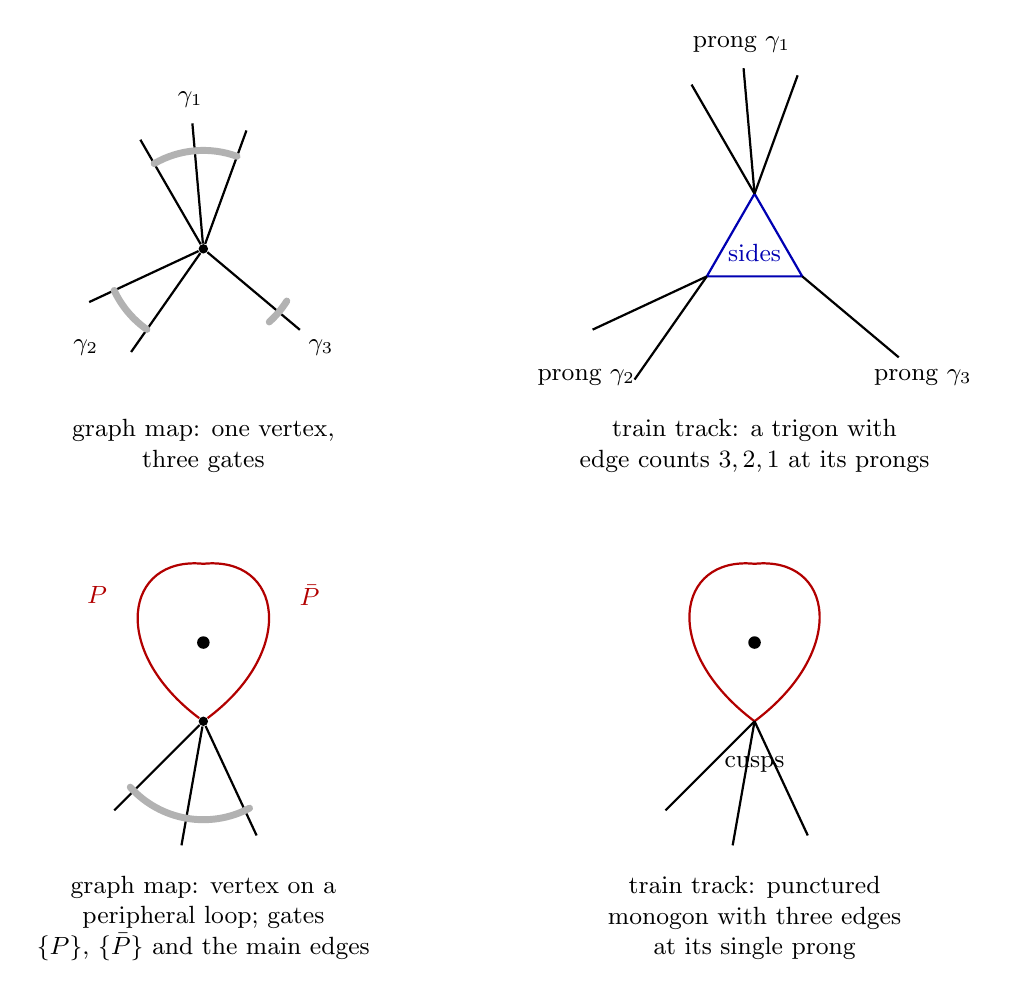
\begin{tikzpicture}[scale=1.0]
    \begin{scope}
      \node[vert] (v) at (0,0) {};
      \foreach \a in {70,95,120} \draw[main] (v) -- (\a:1.6);
      \foreach \a in {205,235} \draw[main] (v) -- (\a:1.6);
      \draw[main] (v) -- (320:1.6);
      \draw[gate] (70:1.25) arc (70:120:1.25);
      \draw[gate] (205:1.25) arc (205:235:1.25);
      \draw[gate] (312:1.25) arc (312:328:1.25);
      \node[lbl] at (95:1.9) {$\gamma_1$};
      \node[lbl] at (220:1.95) {$\gamma_2$};
      \node[lbl] at (320:1.95) {$\gamma_3$};
      \node[lbl,align=center] at (0,-2.5) {graph map: one vertex,\\ three gates};
    \end{scope}
    \begin{scope}[xshift=7cm]
      \coordinate (A) at (90:0.7);
      \coordinate (B) at (210:0.7);
      \coordinate (C) at (330:0.7);
      \draw[side] (A) -- (B) -- (C) -- cycle;
      \foreach \a in {70,95,120} \draw[main] (A) .. controls ($(A)+(\a:0.8)$) .. ($(A)+(\a:1.6)$);
      \foreach \a in {205,235} \draw[main] (B) .. controls ($(B)+(\a:0.8)$) .. ($(B)+(\a:1.6)$);
      \draw[main] (C) .. controls ($(C)+(320:0.8)$) .. ($(C)+(320:1.6)$);
      \node[lbl] at ($(A)+(95:1.9)$) {prong $\gamma_1$};
      \node[lbl] at ($(B)+(220:2.0)$) {prong $\gamma_2$};
      \node[lbl] at ($(C)+(320:2.0)$) {prong $\gamma_3$};
      \node[lbl,blue!70!black] at (0,-0.05) {sides};
      \node[lbl,align=center] at (0,-2.5) {train track: a trigon with\\ edge counts $3,2,1$ at its prongs};
    \end{scope}
    \begin{scope}[yshift=-6cm]
      \node[vert] (v) at (0,0) {};
      \node[punct] at (0,1.0) {};
      \draw[periph] (v) .. controls (-1.2,0.9) and (-1.0,2.1) .. (0,2.0)
                        .. controls (1.0,2.1) and (1.2,0.9) .. (v);
      \node[lbl,red!70!black] at (-1.35,1.6) {$\per$};
      \node[lbl,red!70!black] at (1.35,1.6) {$\anti\per$};
      \foreach \a in {225,260,295} \draw[main] (v) -- (\a:1.6);
      \draw[gate] (222:1.25) arc (222:298:1.25);
      \node[lbl,align=center] at (0,-2.5) {graph map: vertex on a\\ peripheral loop; gates\\ $\set{\per}$, $\set{\anti\per}$ and the main edges};
    \end{scope}
    \begin{scope}[xshift=7cm,yshift=-6cm]
      \coordinate (c) at (0,0);
      \node[punct] at (0,1.0) {};
      \draw[periph] (c) .. controls (-1.2,0.9) and (-1.0,2.1) .. (0,2.0)
                        .. controls (1.0,2.1) and (1.2,0.9) .. (c);
      \foreach \a in {225,260,295} \draw[main] (c) .. controls ($(c)+(\a:0.9)$) .. (\a:1.6);
      \node[lbl] at (0,-0.55) {cusps};
      \node[lbl,align=center] at (0,-2.5) {train track: punctured\\ monogon with three edges\\ at its single prong};
    \end{scope}
  \end{tikzpicture}
  \caption{The blow-up.  Top: a graph-map vertex with three gates is the
    same object as a trigon whose corners are the prongs and whose sides
    are infinitesimal edges.  Bottom: a puncture; the peripheral loop
    $\per$ is a real edge of the graph, and in \ttauto\ it is the side of
    the punctured monogon.  The main edges at the single prong are pairwise
    separated by cusps.}
  \label{fig:blowup}
\end{figure}

\begin{table}[h]
  \centering
  \begin{tabular}{@{}ll@{}}
    \toprule
    Bestvina--Handel & \ttauto \\
    \midrule
    vertex $v$ & an unpunctured multigon, taken as a whole; \\
               & or \emph{one prong} of a punctured multigon \\
    direction at $v$ & a signed main letter with tail at $v$; \\
                     & at a punctured prong also the two directions
                       $\per,\anti\per$ of its sides \\
    gate at $v$ & a prong (a priori); refined by $\Dg^k$-coincidence \\
    infinitesimal edge & a side of an \emph{unpunctured} multigon that
                         some iterate traverses \\
    peripheral edge & a side of a \emph{punctured} multigon (the loop of a
                      monogon) \\
    $M_H$ & the transition matrix on the $n$ main edges \\
    turn taken by $g^k(e)$ & consecutive main letters $x\,S\,y$ of an image
                             word, joining $\anti x$ to $y$ \\
    \bottomrule
  \end{tabular}
  \caption{The dictionary.  A side of a punctured multigon is a real
    (peripheral) edge of $G$, so its two ends are two different vertices
    when $k\ge2$ and the same vertex when $k=1$.}
  \label{tab:dictionary}
\end{table}

The peripheral subgraph is the set of sides of punctured multigons, the
main edges are $H$, and a subword $x\,S\,y$ of an image word contributes
the turn $(\anti x,y)$ at the multigon of $S$ if $S$ is a side of an
unpunctured multigon, or the two turns $(\anti x,S)$ at the tail prong
of $S$ and $(\anti S,y)$ at its head prong if $S$ is peripheral.  Three
consequences of the dictionary do most of the work.

\begin{Lemma}
  \label{lem:refine}
  Gates refine prongs: two directions at different prongs of the same
  multigon are never equivalent.
\end{Lemma}
\begin{proof}
  A fold detaches one end of an edge from a prong and re-attaches it at
  a prong of another multigon; it never changes the number of prongs of
  any multigon.  So along a folding path the prongs of the start track
  are mapped bijectively to the prongs of the end track
  (\code{prong_image}), and $\Dg^k(E)$ has its tail at the image prong
  of the tail of $E$.  Directions at different prongs have images at
  different prongs, hence never coincide.
\end{proof}

\begin{Lemma}
  \label{lem:alternate}
  Every image word of a main edge under a composed fold map alternates
  main letters and side letters, begins and ends with a main letter, and
  never contains two consecutive side letters.
\end{Lemma}
\begin{proof}
  A single fold maps every main edge either to a single main letter or to
  $x\,S\,y$ with $x,y$ main and $S$ a side (Section~\ref{sec:onefold});
  sides map to single sides.  Substituting such words into such words
  preserves the pattern.
\end{proof}

\begin{Corollary}[efficiency is automatic]
  \label{cor:efficient}
  Every realised turn joins two different prongs, hence two different
  gates: the graph maps produced by folding paths are efficient.
\end{Corollary}
\begin{proof}
  By Lemma~\ref{lem:alternate} a turn is always $x\,S\,y$ with $S$ a
  side from one prong to the next; so $\anti x$ and $y$ are at different
  prongs of that multigon, and by Lemma~\ref{lem:refine} in different
  gates.
\end{proof}

\begin{Corollary}[the test at a puncture]
  \label{cor:puncture}
  Let $v$ be a prong of a punctured multigon, with incoming peripheral
  side $\per_{\mathrm{in}}$, outgoing peripheral side
  $\per_{\mathrm{out}}$, and main gates $\mu_1,\dots,\mu_r$ in cyclic
  order between them.  The only infinitesimal edges that can be realised
  at $v$ are $\anti\per_{\mathrm{in}}$--$\mu_1$ and
  $\mu_r$--$\per_{\mathrm{out}}$.  Hence the gate graph at $v$ is
  connected if and only if $r=1$ and both of these turns are taken by
  some iterate.
\end{Corollary}
\begin{proof}
  A turn joining two main gates at the same prong would be a turn inside
  a prong, excluded by Lemma~\ref{lem:alternate}.  A turn joining
  $\anti\per_{\mathrm{in}}$ to $\per_{\mathrm{out}}$ would need two
  consecutive peripheral letters, also excluded; images of peripheral
  edges are single letters and take no turns.  So at most the two named
  edges exist, and they connect all $r+2$ gates only when $r=1$.
\end{proof}

At a punctured monogon this says: the map is reducible at that puncture
either because the prong is \emph{refined}, two of its main edges never
having their cusp folded so that they stay in different gates, or because
the loop is never traversed in one of its two senses.  When the test
passes, the infinitesimal edges at the prong form the path
$\anti\per$--$\mu$--$\per$, the triangle with one side missing of
Proposition~\ref{prop:shape}.

\begin{Corollary}
  \label{cor:unpunctured}
  At an unpunctured $k$-gon with connected gate graph, at most one prong
  is refined, and then into exactly two gates.
\end{Corollary}
\begin{proof}
  Two gates in the same prong are adjacent in the cyclic order and cannot
  be joined (Lemma~\ref{lem:alternate}), so each refined prong costs one
  missing side of the polygon on the gates, and
  Proposition~\ref{prop:shape} allows at most one.
\end{proof}

\subsection{The criterion as implemented}
Putting the pieces together, \code{record_pA} accepts a closed path
$\gamma$ as pseudo-Anosov when
\begin{enumerate}
  \item $M(\gamma)$ is primitive;
  \item its Perron root $\lam$, found by Newton iteration on the
    characteristic polynomial from the upper bound $\min(\max$ row sum,
    $\max$ column sum$)$, lies in the requested window
    (\code{min_dilatation}, \code{max_dilatation});
  \item at every Bestvina--Handel vertex of $\trk$, unpunctured multigon
    or prong of a punctured multigon, the gates of $g(\gamma)$ are
    connected by the realised turns.
\end{enumerate}
Condition~3 is \code{folding_path::gates().connected}; the next section
explains how it is computed.  The analysis also reports whether every
vertex has one of the shapes of Proposition~\ref{prop:shape}
(\code{shapes_ok}); this is not used to accept or reject, only printed,
since by Theorem~\ref{thm:bh} it must hold whenever condition~3 does.

%======================================================================
\section{Computing the condition along a path}
\label{sec:computing}

The image words of $g(\gamma)$ have length of order $\lam^L$, so composing
words in the search is out of the question.  The gate test needs only
two things from $g$: its derivative $\Dg g$ on directions, and the set
$\turns(g)$ of turns taken by the images of the main edges.  Both
compose without words.

\subsection{Derivative data of one fold}
For a one-step map $h$ (three-letter words at most) with target
numbering $N$, the struct \code{fold_derivative(AM, N)} records
\begin{itemize}
  \item $\Dg h$ on every signed letter, main and side (\code{apply});
    for a side letter this is just the image side;
  \item $\turns(h)$: for each main edge whose image is $x\,S\,y$, the
    turn $(\anti x,y)$ at the unpunctured multigon of $S$, or the turns
    $(\anti x,S)$ and $(\anti S,y)$ if $S$ is peripheral, all in the
    letters of $N$.
\end{itemize}
The constructor checks that consecutive letters of each word share a
prong of $N$ and that no turn falls inside a prong, and fails fast
otherwise; these are the invariants of Section~\ref{sec:onefold}.

\subsection{Composition}
Write $g$ for the map composed so far and $h$ for the next one-step map,
so the new composite is $g\circ h$ (substitute $g$ into the letters of
$h$).

\begin{Lemma}
  \label{lem:compose}
  $\Dg(g\circ h)=\Dg g\circ\Dg h$ and
  $\turns(g\circ h)=\turns(g)\cup\Dg g\bigl(\turns(h)\bigr)$, where
  $\Dg g$ acts on a turn componentwise.
\end{Lemma}
\begin{proof}
  The first letter of $g(h(e))$ is the first letter of $g$ applied to the
  first letter of $h(e)$.  For the turns, write $h(e)=x_1S_1x_2\cdots$;
  then $g(h(e))=g(x_1)\,g(S_1)\,g(x_2)\cdots$.  The turns inside each
  $g(x_i)$ belong to $\turns(g)$, and every main letter of the middle
  track occurs as some $x_i$ since the permutation part of a fold is a
  bijection, so all of $\turns(g)$ is picked up.  Each $g(S_i)$ is a
  single side and contributes no turn.  The turn between the last letter
  of $g(x_i)$ and the first letter of $g(x_{i+1})$ is
  $(\Dg g(\anti{x_i}),\Dg g(x_{i+1}))$, the image of the turn
  $(\anti{x_i},x_{i+1})$ of $h$.  Peripheral sides behave the same way,
  with $\Dg g(S)=g(S)$.
\end{proof}

The class \code{gate_accumulator} holds the pair $(\Dg g,\turns(g))$ and
\code{push_back(d)} replaces it by
$(\Dg g\circ\Dg h,\ \turns(g)\cup\Dg g(\turns(h)))$; a \code{folding_path}
of length $L$ is processed in $O(L\,(n+n_{\mathrm{s}}))$ operations.

\subsection{Gates and connectivity}
With the composed $(\Dg g,\turns(g))$ of a closed path read as a self-map
of the start track with numbering $N$, \code{analyse(N)} does the
following at each Bestvina--Handel vertex.
\begin{enumerate}
  \item The directions are the prong letters of the vertex's prongs, plus
    $\anti{\per_{\mathrm{in}}}$ and $\per_{\mathrm{out}}$ at a punctured
    prong, in cyclic order.
  \item Gates: two directions are equivalent when $\Dg^K$ identifies
    them, where $K$, the square of the number of directions, bounds the
    pre-period of the finite dynamical system $\Dg$ on the direction set.
    Gates are checked to be consecutive blocks.
  \item Realised turns of all iterates: $\turns(g^k)=\bigcup_{j<k}
    (\Dg g)^j\,\turns(g)$, so the closure of $\turns(g)$ under
    $\Dg g\times\Dg g$ is computed, a finite computation on at most
    $(2n+2n_{\mathrm{s}})^2$ pairs.
  \item Each realised turn at the vertex joins the gates of its two
    directions; a union-find over the gates gives the number of
    components.  A realised turn inside a gate, or a turn whose two
    directions are at different vertices, is an invariant violation and
    fails fast.
  \item The infinitesimal-edge pattern is compared with
    Proposition~\ref{prop:shape}.
\end{enumerate}
The result is a \code{gate_analysis}: a flag \code{connected} for the
whole map, \code{shapes_ok}, and one \code{gate_vertex_report} per
vertex with its directions, gates, joins and component count, printable
with \code{print}.  A word-based implementation \code{analyse_gates(N, AM)},
which reads a fully composed map, exists for cross-checking and agrees
with the accumulator on every path the tests try.

\subsection{Why composing across vertices needs no transport}
\label{sec:labels}
The one-step map stored at a branch has its target letters in the
numbering of the fold result, a track object that was normalised and
then identified with a stored vertex by coding equality.  The next
branch, and the accumulator's final \code{analyse}, use the numbering of
the \emph{stored} vertex.  These agree exactly, because the numbering is
a function of the coding (Section~\ref{sec:numbering}): identifying the
two tracks ``by number'' is the identity on labels and an isomorphism of
labelled tracks.  This holds even at a track with a nontrivial cyclic
symmetry, where several uncusped monogons give the same minimal coding:
the symmetry maps one minimising monogon to another and the numbering to
itself, so it makes no difference which minimiser \code{normalise()}
puts in slot~$0$.  Consequently the composed matrix and the composed
derivative data describe the same homeomorphism, the folds closed up by
the canonical identification, and the accumulator can be fed the stored
one-step maps directly.

(Closing up a path at a cyclically symmetric track by the symmetry
instead gives a different mapping class; the automaton does not
enumerate those separately, and \cite[\S ``Cyclic symmetry'']{Lanneau2011}
argues that folding at symmetry-related cusps already produces them.  The
gate test inherits this convention.)

%======================================================================
\section{A four-puncture example, worked in full}
\label{sec:example}

\subsection{The stratum and its automaton}
Take the disc with $\np=4$ punctures and the stratum $1.\,1.\,1.\,1.\,(2)$:
four punctured monogons and a 2-pronged singularity on the outer
boundary (Figure~\ref{fig:tracks}, left).
Every track on it has $n=3$ main edges and $n_{\mathrm{s}}=4$ prongs, so
the letters are $1,2,3$ (edges) and $4,5,6,7$ (the four loops).  The
automaton has four vertices (Figure~\ref{fig:automaton}).  Vertex~0 is
the track whose four monogons carry $1,1,1,3$ edges; vertices $1$, $2$
and $3$ have monogons with $1,1,2,2$ edges and differ in how the edges
are arranged.  Vertex~1 is a dead end: its two branches are loops at
itself and its matrices are permutations plus one, never primitive, so
no closed path through it is a candidate.  This is the one
``non-pseudo-Anosov'' track of the stratum; the main automaton is
$\set{0,2,3}$.

\begin{figure}[t]
  \centering
  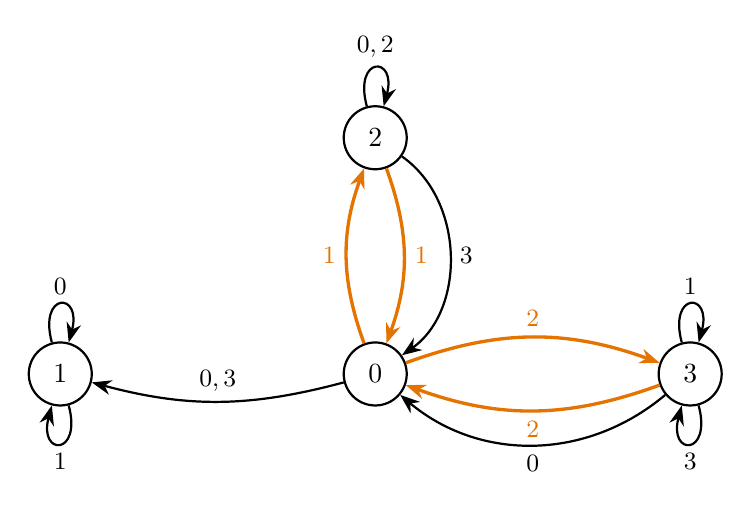
\begin{tikzpicture}[scale=1.0,>=Stealth]
    \node[state] (v0) at (0,0) {$0$};
    \node[state] (v1) at (-4,0) {$1$};
    \node[state] (v2) at (0,3) {$2$};
    \node[state] (v3) at (4,0) {$3$};
    % vertex 0 -> 1 (branches 0 and 3)
    \draw[branch] (v0) to[bend left=15] node[lbl,above] {$0,3$} (v1);
    % vertex 0 -> 2 (branch 1) and 2 -> 0 (branch 1): the cycle
    \draw[cyc] (v0) to[bend left=20] node[lbl,left] {$1$} (v2);
    \draw[cyc] (v2) to[bend left=20] node[lbl,right] {$1$} (v0);
    \draw[branch] (v2) to[bend left=55] node[lbl,right] {$3$} (v0);
    % vertex 0 -> 3 (branch 2) and 3 -> 0 (branch 2)
    \draw[cyc] (v0) to[bend left=20] node[lbl,above] {$2$} (v3);
    \draw[cyc] (v3) to[bend left=20] node[lbl,below] {$2$} (v0);
    \draw[branch] (v3) to[bend left=40] node[lbl,below] {$0$} (v0);
    % self loops
    \draw[branch] (v1) to[loop above] node[lbl] {$0$} (v1);
    \draw[branch] (v1) to[loop below] node[lbl] {$1$} (v1);
    \draw[branch] (v2) to[loop above] node[lbl] {$0,2$} (v2);
    \draw[branch] (v3) to[loop above] node[lbl] {$1$} (v3);
    \draw[branch] (v3) to[loop below] node[lbl] {$3$} (v3);
  \end{tikzpicture}
  \caption{The folding automaton of the four-puncture stratum
    $1.\,1.\,1.\,1.\,(2)$.  Arrows are labelled by branch index; the
    thick orange arrows form the closed path $0\to2\to0\to3\to0$ with
    branches $1,1,2,2$ analysed below.  Vertex~1 supports no
    pseudo-Anosov.  (The arrow $2\to0$ with branch~$1$ and the arrow
    $3\to0$ with branch~$2$ are drawn separately from the branches $3$
    and $0$ to the same targets.)}
  \label{fig:automaton}
\end{figure}

\subsection{The numbering of vertex~0}
The canonical numbering of the track at vertex~0 is:
\begin{center}
  \small
  \begin{tabular}{@{}cllc@{}}
    \toprule
    prong & multigon & directions (prong letters) & loop \\
    \midrule
    0 & monogon 0, one edge    & $1$              & $4$ \\
    1 & monogon 3, three edges & $\anti1,\,2,\,3$ & $5$ \\
    2 & monogon 1, one edge    & $\anti2$         & $6$ \\
    3 & monogon 2, one edge    & $\anti3$         & $7$ \\
    \bottomrule
  \end{tabular}
\end{center}
Edge $1$ runs from prong $0$ to prong $1$, edge $2$ from prong $1$ to
prong $2$, edge $3$ from prong $1$ to prong $3$.  The two cusps are both
at prong~1, between edges $\anti1$ and $2$ (fold indices $0,1$) and
between $2$ and $3$ (fold indices $2,3$).  The Bestvina--Handel vertices
are the four prongs, each a puncture.

\subsection{The four folds}
The closed path starts at vertex~0 and takes branches $1,1,2,2$, visiting
$0,2,0,3,0$.  The fold records read off the library are:
\begin{center}
  \small
  \begin{tabular}{@{}clcccl@{}}
    \toprule
    step & at vertex & fold & moved onto & target $t\to t'$ & image of moved edge \\
    \midrule
    0 & 0 & index 1 (dir $-1$) & $2$ onto $1$ & $1\to1$ & $2\mapsto \anti2\,\anti5\,\anti1$ \\
    1 & 2 & index 1 (dir $-1$) & $1$ onto $2$ & $1\to1$ & $1\mapsto \anti3\,5\,\anti1$ \\
    2 & 0 & index 2 (dir $+1$) & $2$ onto $3$ & $2\to2$ & $2\mapsto 2\,6\,3$ \\
    3 & 3 & index 2 (dir $+1$) & $3$ onto $2$ & $1\to1$ & $3\mapsto \anti3\,5\,\anti1$ \\
    \bottomrule
  \end{tabular}
\end{center}
In each case the target is a punctured monogon, so $t'=t$ and the side
letter is that monogon's loop, traversed positively or negatively.  The
complete one-step maps, each on the seven letters and each written in
the numbering of its target vertex, are
\begin{align*}
  h_0&: & 1&\mapsto 2, & 2&\mapsto \anti2\,\anti5\,\anti1, & 3&\mapsto 3,
       & 4&\mapsto 5, & 5&\mapsto 6, & 6&\mapsto 4, & 7&\mapsto 7;\\
  h_1&: & 1&\mapsto \anti3\,5\,\anti1, & 2&\mapsto 1, & 3&\mapsto 2,
       & 4&\mapsto 7, & 5&\mapsto 4, & 6&\mapsto 5, & 7&\mapsto 6;\\
  h_2&: & 1&\mapsto 1, & 2&\mapsto 2\,6\,3, & 3&\mapsto 2,
       & 4&\mapsto 4, & 5&\mapsto 5, & 6&\mapsto 7, & 7&\mapsto 6;\\
  h_3&: & 1&\mapsto \anti2, & 2&\mapsto 3, & 3&\mapsto \anti3\,5\,\anti1,
       & 4&\mapsto 6, & 5&\mapsto 5, & 6&\mapsto 7, & 7&\mapsto 4.
\end{align*}
Each side letter is permuted (the prongs are carried bijectively), each
unmoved edge is relabelled with a sign, and the moved edge goes to a
three-letter path whose middle letter is a side of the target.

\subsection{The composed map and its matrix}
Composing, $g=h_3\circ h_2\circ h_1\circ h_0$ is
\begin{align*}
  1&\mapsto \anti2, &
  2&\mapsto 2\,\anti6\,\anti2\,\anti5\,3, &
  3&\mapsto 3\,7\,\anti3\,5\,\anti1, \\
  4&\mapsto 6, & 5&\mapsto 5, & 6&\mapsto 7, & 7&\mapsto 4.
\end{align*}
Every image alternates main and side letters and is an edge path in the
track at vertex~0 (check with the table above: $\anti2$ ends at prong~1,
side $6$ is the loop at prong~2 which is where $\anti2$ ends, and so on).
Counting main letters gives the transition matrix and its characteristic
polynomial,
\[
  M(\gamma)=\begin{pmatrix} 0&0&1\\ 1&2&0\\ 0&1&2 \end{pmatrix},
  \qquad
  \det(xI-M)=x^3-4x^2+4x-1=(x-1)(x^2-3x+1),
\]
with $M^2>0$, so $M$ is primitive with Perron root
$\lam=\varphi^2=2.61803$.  By the matrix conditions alone this path is a
pseudo-Anosov of dilatation $2.61803$.

\subsection{Derivative, turns, gates}
The derivative $\Dg g$ on the fourteen directions is read off the first
letters:
\[
  \begin{array}{c|ccccccc}
    E & 1 & 2 & 3 & 4 & 5 & 6 & 7 \\ \hline
    \Dg g(E) & \anti2 & 2 & 3 & 6 & 5 & 7 & 4
  \end{array}
  \qquad
  \begin{array}{c|ccccccc}
    E & \anti1 & \anti2 & \anti3 & \anti4 & \anti5 & \anti6 & \anti7 \\ \hline
    \Dg g(E) & 2 & \anti3 & 1 & \anti6 & \anti5 & \anti7 & \anti4
  \end{array}
\]
(the image of $\anti e$ is the inverse of the image of $e$, so
$\Dg g(\anti e)$ is the inverse of the last letter of $g(e)$).  The turns
taken by the three image words, recorded at the target prongs, are
\[
  \turns(g)=\set{(\anti2,\anti6),\ (\anti6,\anti2),\ (\anti5,2),\ (\anti5,3)\ \text{from } g(2);\quad
  (\anti3,7),\ (\anti7,\anti3),\ (\anti5,\anti1),\ (3,5)\ \text{from } g(3)}
\]
where, following the dictionary, a subword $x\,S\,y$ with $S$ a loop
contributes $(\anti x,S)$ and $(\anti S,y)$; the library stores the seven
distinct unordered pairs $(\anti7,\anti3)$, $(\anti6,\anti2)$,
$(\anti5,\anti1)$, $(\anti5,2)$, $(\anti3,7)$, $(\anti2,6)$, $(3,5)$.
Closing under $\Dg g\times\Dg g$ adds nothing new here.  The gates at
each prong are the classes under $\Dg g^K$, and the joins are the
realised turns between distinct gates:

\begin{center}
  \small
  \begin{tabular}{@{}llll@{}}
    \toprule
    vertex & gates & joins & connected \\
    \midrule
    prong 0 (monogon 0) & $\set{\anti4},\set{1},\set{4}$ & $\anti4\!\sim\!1,\ 1\!\sim\!4$ & yes \\
    prong 1 (monogon 3) & $\set{\anti5},\set{\anti1,2},\set{3},\set{5}$
       & $\anti5\!\sim\!\anti1,\ \anti5\!\sim\!2,\ 3\!\sim\!5$ & \textbf{no} (2 components) \\
    prong 2 (monogon 1) & $\set{\anti6},\set{\anti2},\set{6}$ & $\anti6\!\sim\!\anti2,\ \anti2\!\sim\!6$ & yes \\
    prong 3 (monogon 2) & $\set{\anti7},\set{\anti3},\set{7}$ & $\anti7\!\sim\!\anti3,\ \anti3\!\sim\!7$ & yes \\
    \bottomrule
  \end{tabular}
\end{center}

At the three one-edge monogons the gate graph is the path
$\anti\per$--$\mu$--$\per$ of Corollary~\ref{cor:puncture}: connected.  At
prong~1 the three main directions $\anti1,2,3$ fall into two gates, since
$\Dg g$ sends $\anti1\mapsto2\mapsto2$ while $3\mapsto3$: the cusp
between $2$ and $3$ is never folded along this path, and no iterate
identifies them.  The loop $5$ is fixed by $g$, and its two ends are
joined to different gates: $\anti5$ to $\set{\anti1,2}$ and $5$ to
$\set{3}$.  The gate graph has the two components $\set{\anti5,\anti1,2}$
and $\set{3,5}$ (Figure~\ref{fig:badvertex}), so by Theorem~\ref{thm:bh}
$\ho$ is reducible, and \code{record_pA} moves this path to the rejected
list.  What is going on is visible in the map: $g$ fixes the loop~$5$,
so the puncture inside monogon~3 is fixed and the homeomorphism is the
golden-mean pseudo-Anosov $\sigma_1\sigma_2^{-1}$ of the three-punctured
disc (dilatation $\varphi^2$, the minimum for $\np=3$) with a fourth
puncture standing still; a curve enclosing that puncture and its
neighbour along the fixed gap is invariant.

\begin{figure}[t]
  \centering
  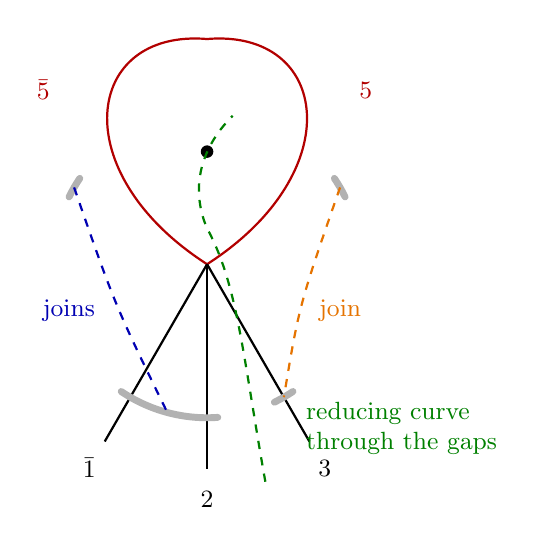
\begin{tikzpicture}[scale=1.3]
    \coordinate (c) at (0,0);
    \node[punct] at (0,1.1) {};
    % loop 5 around the puncture: leaves to the right (5), returns from the left (-5)
    \draw[periph] (c) .. controls (1.4,0.9) and (1.2,2.3) .. (0,2.2)
                     .. controls (-1.2,2.3) and (-1.4,0.9) .. (c);
    \node[lbl,red!70!black] at (1.55,1.7) {$5$};
    \node[lbl,red!70!black] at (-1.6,1.7) {$\anti5$};
    % three main edges below: -1, 2, 3 from left to right
    \draw[main] (c) -- (240:2.0);
    \draw[main] (c) -- (270:2.0);
    \draw[main] (c) -- (300:2.0);
    \node[lbl] at (240:2.3) {$\anti1$};
    \node[lbl] at (270:2.3) {$2$};
    \node[lbl] at (300:2.3) {$3$};
    % gates: {-5} at ~150, {-1,2} spanning 240-270, {3} at 300, {5} at ~30
    \draw[gate] (236:1.5) arc (236:274:1.5);
    \draw[gate] (296:1.5) arc (296:304:1.5);
    \draw[gate] (146:1.5) arc (146:154:1.5);
    \draw[gate] (26:1.5) arc (26:34:1.5);
    % joins: -5 ~ {-1,2} (two turns), 3 ~ 5
    \draw[chord,blue!70!black] (150:1.5) .. controls (-0.9,-0.4) .. (255:1.5);
    \draw[chord,orange!90!black] (30:1.5) .. controls (0.9,-0.4) .. (300:1.5);
    \node[lbl,blue!70!black] at (-1.35,-0.45) {joins};
    \node[lbl,orange!90!black] at (1.3,-0.45) {join};
    % reducing curve: enters between edges 2 and 3, leaves the vertex into
    % the sector between the two ends of the loop (the puncture's side)
    \draw[thick,dashed,green!50!black] (285:2.2) .. controls (0.35,-0.9) and (0.3,-0.2) .. (0,0.35)
      .. controls (-0.15,0.7) and (-0.1,1.1) .. (0.25,1.45);
    \node[lbl,green!50!black,align=left] at (1.9,-1.6) {reducing curve\\ through the gaps};
  \end{tikzpicture}
  \caption{The gate graph at prong~1 of vertex~0 (the fixed three-edge
    punctured monogon).  Five directions in cyclic order:
    $\anti5,\anti1,2,3,5$.  Four gates (grey arcs): the main prong is
    refined into $\set{\anti1,2}$ and $\set{3}$.  The realised turns join
    $\anti5$ to $\set{\anti1,2}$ and $3$ to $5$; nothing joins the two
    halves.  A reducing curve passes through the vertex between the gates
    $\set{\anti1,2}$ and $\set{3}$ and leaves it in the sector between the
    two ends of the loop, on the puncture's side.}
  \label{fig:badvertex}
\end{figure}

\subsection{The genuine class with the same dilatation}
The same stratum has a genuine pseudo-Anosov of dilatation $2.61803$,
the minimum of the stratum: for instance the path $0\to2\to0\to3\to0$
with branches $1,1,2,0$, differing from the rejected one only in its last
fold, has matrix with characteristic polynomial $x^3-2x^2-2x+1$ and
passes the gate test at all four prongs.  Both matrices are primitive
with the same spectral radius; the matrix conditions cannot separate
them, and the two classes sit side by side in the search's accepted and
rejected lists.

%======================================================================
\section{Using it}
\label{sec:api}

The gate test is on by default in \code{ttauto::ttauto::search()};
\code{check_gates(false)} restores the matrix-only behaviour.  After a
search, \code{pA_list()} holds the accepted classes and
\code{rejected_pA_list()} the classes rejected by the gate test, both
keyed by characteristic polynomial; \code{gate_candidates()},
\code{gate_rejected()} and \code{gate_rejection_rate()} count the
closed paths that reached the test (primitive matrix, dilatation in the
window) and how many failed.  The statistics block printed at the end of
a search contains a line
{\footnotesize
\begin{verbatim}
      Gate test          = 3 rejected of 47 candidates (6.38%) (cumulative)
\end{verbatim}}
To inspect one path, build it as a \code{folding_path} and call
\code{gates()}; the following program reproduces
Section~\ref{sec:example}.
{\footnotesize
\begin{verbatim}
#include <iostream>
#include "traintracks/build.hpp"
#include "traintracks/gates.hpp"
#include "traintracks/traintrack.hpp"
#include "ttauto/folding_path.hpp"
#include "ttauto/ttauto.hpp"
#include "ttauto/ttfoldgraph.hpp"
using traintracks::traintrack;

int main()
{
  auto ttv = traintracks::build_traintrack_list(4);   // strata for n=4
  ttauto::ttfoldgraph<traintrack> ttg(ttv[0]);        // stratum 1.1.1.1.(2)

  ttauto::folding_path<traintrack> p(ttg,0);          // start at vertex 0
  for (int b : {1,1,2,2}) p.push_back(b);             // branches
  std::cout << p.transition_matrix() << p.traintrack_map();
  p.gates().print(std::cout);                          // the gate table

  ttauto::ttauto<traintrack> tta(ttg);
  tta.max_pathlength(4).badword_length(0);
  tta.search();
  tta.print_pA_list();                                 // accepted classes
  tta.print_rejected_pA_list();                        // the (x-1)(x^2-3x+1) class
}
\end{verbatim}}
The one-step data of branch $b$ at vertex $v$ is available as
\code{ttg.traintrack_map(v,b)} and \code{ttg.transition_matrix(v,b)}.
The fold record of a single fold is filled by
\code{tt.fold_with_map(f, fm)} and printed by \code{fm.print(std::cout)};
the numbering of any track by \code{tt.numbering().print(std::cout)}.

%======================================================================
\appendix
\section{Concept to code}
\label{sec:appendix}

\begin{center}
  \footnotesize
  \begin{tabular}{@{}>{\raggedright\arraybackslash}p{0.25\textwidth}>{\raggedright\arraybackslash}p{0.37\textwidth}>{\raggedright\arraybackslash}p{0.31\textwidth}@{}}
    \toprule
    concept & where & pinned by \\
    \midrule
    multigons, prongs, cusps, folds &
      \code{include/traintracks/multigon.hpp}, \code{traintrack.hpp};
      \code{lib/traintracks/traintrack.cpp} &
      \code{testsuite/traintracks/test_traintrack_core.cpp} \\
    codings, normal form, symmetries &
      \code{include/traintracks/coding.hpp}; \code{lib/traintracks/coding.cpp} &
      \code{test_traintrack_core.cpp} \\
    canonical numbering (\code{ttnumbering}) &
      \code{coding.hpp}, \code{coding.cpp} &
      \code{test_numbering.cpp} (order agrees with \code{weights()}; labels
      are a function of the coding, also at symmetric vertices) \\
    fold record, one-step map, one-step matrix &
      \code{include/traintracks/fold_map.hpp}; \code{lib/traintracks/fold_map.cpp};
      \code{map.hpp} &
      \code{test_map_consistency.cpp}, \code{test_fold_map_paths.cpp}
      (words are edge paths, abelianise to the matrix) \\
    letter conventions &
      \code{include/traintracks/map_labels.hpp} & \code{test_map_consistency.cpp} \\
    permutation-plus-one matrices &
      \code{include/traintracks/mathmatrix_permplus1.hpp} &
      \code{test_mathmatrix_permplus1.cpp} \\
    strata representatives &
      \code{include/traintracks/build.hpp}; \code{lib/traintracks/build.cpp} &
      \code{test_traintrack_core.cpp} \\
    derivative data, accumulator, gate test &
      \code{include/traintracks/gates.hpp}; \code{lib/traintracks/gates.cpp} &
      \code{test_gates.cpp} (the $n=4$ example, the $n=6$ case,
      exhaustive sweeps) \\
    automaton &
      \code{include/ttauto/ttfoldgraph.hpp} &
      \code{test_map_consistency.cpp}, \code{test_fold_map_paths.cpp} \\
    folding paths, \code{gates()} &
      \code{include/ttauto/folding_path.hpp} &
      \code{testsuite/ttauto/test_folding_path_and_badwords.cpp} \\
    search, acceptance, primitivity, rejected list &
      \code{include/ttauto/ttauto.hpp} (\code{record_pA}) &
      \code{test_ttauto_search.cpp}, \code{test_ttauto_gates.cpp},
      \code{test_min_dilatations.cpp} \\
    classes of pseudo-Anosovs &
      \code{include/ttauto/pAclass.hpp} & \code{test_ttauto_search.cpp} \\
    bad words & \code{include/ttauto/badwords.hpp} &
      \code{test_folding_path_and_badwords.cpp} \\
    rejection census over strata &
      \code{tests/ttauto_gate_census.cpp} & (diagnostic program) \\
    \bottomrule
  \end{tabular}
\end{center}

\noindent
Test programs live under \code{testsuite/traintracks/} and
\code{testsuite/ttauto/} and run with \code{ctest --test-dir build}.
They are described in \code{TESTING.md} and \code{testsuite/COVERAGE.md};
\code{CODE_STRUCTURE.md} gives a class-by-class tour of the code.

\begin{thebibliography}{9}
\bibitem{Bestvina1995} M.~Bestvina and M.~Handel, \emph{Train-tracks for
  surface homeomorphisms}, Topology \textbf{34} (1995), 109--140.
\bibitem{HallBHchapter} T.~Hall, \emph{The Bestvina--Handel algorithm},
  unpublished book chapter, \S3 (derivative, gates, efficiency).
\bibitem{HallTrain} T.~Hall, \emph{Trains: a C++ program for computing
  train tracks of surface homeomorphisms},
  \url{http://www.liv.ac.uk/~tobyhall/T_Hall.html}.
\bibitem{Lanneau2011} E.~Lanneau and J.-L. Thiffeault, \emph{Enumerating
  pseudo-Anosov homeomorphisms of punctured discs}, manuscript
  (\code{pubs/ttauto paper/ttauto.tex}).
\bibitem{Lanneau2011b} E.~Lanneau and J.-L. Thiffeault, \emph{On the
  minimum dilatation of braids on the punctured disc}, Geom. Dedicata
  \textbf{152} (2011), 165--182.
\bibitem{Ham2007} J.-Y. Ham and W.~T. Song, \emph{The minimum dilatation
  of pseudo-Anosov 5-braids}, Experiment. Math. \textbf{16} (2007),
  167--179.
\bibitem{Song2002} W.~T. Song, K.~H. Ko and J.~E. Los, \emph{Entropies of
  braids}, J. Knot Theory Ramifications \textbf{11} (2002), 647--666.
\end{thebibliography}

\end{document}
